\documentclass[12pt,a4paper,twoside]{article}

\usepackage[utf8]{inputenc}
\usepackage[T1]{fontenc}
\usepackage{amsmath,amssymb,amsthm}
\usepackage{libertine}
\usepackage{fourier}
\usepackage{graphicx}
\usepackage{framed}

\setlength{\voffset}{-28.4mm}
\setlength{\hoffset}{-1in}
\setlength{\topmargin}{20mm}
\setlength{\oddsidemargin}{25mm}
\setlength{\evensidemargin}{25mm}
\setlength{\textwidth}{160mm}

\setlength{\parindent}{0pt}

\setlength{\textheight}{235mm}
\setlength{\footskip}{20mm}
\setlength{\headsep}{50pt}
\setlength{\headheight}{0pt} 

\newcommand\var[1]{{\operatorname{#1}}}
% \var{eval}
% \var{span}
% \var{Hom}
% \var{Der}
% Composition = .
% \delta_{i,j} Kronecher delta
\newcommand\Z[1]{\nicefrac{\integers}{#1\integers}}

%% General things
%       
        \newcommand\mkset[2]{\left\lbrace#1\,|\, #2\right\rbrace}
        \DeclareMathOperator\diag{\text{diag}}

% Number Sets
%
        \DeclareMathOperator\naturals{\mathbb N_0}
        \DeclareMathOperator\posnats{\mathbb N_{>0}}
        \DeclareMathOperator\integers{\mathbb Z}
        \DeclareMathOperator\rationals{\mathbb Q}
        \DeclareMathOperator\reals{\mathbb R}
        \DeclareMathOperator\complex{\mathbb C}

% Definitional Equality
%
        \DeclareMathOperator\defeq{\overset{\text{def}}=}


% Standard Varieties and related constructions
%
        \DeclareMathOperator\proj{\mathbb P}
        % projective variety for some ideal
        \DeclareMathOperator\V{\mathcal V}
        \DeclareMathOperator\I{\mathcal I}


% Morphism Arrows
%
        \newcommand\hookr\hookrightarrow  
        \newcommand\hookl\hookleftarrow  

%% Polynomial things
%
        \DeclareMathOperator\del\partial



\newtheorem{dummy}{dummy}[section]
\newtheorem{proposition}[dummy]{Proposition}
\newtheorem{corollary}[dummy]{Corollary}
\newtheorem{theorem}[dummy]{Theorem}
\newtheorem{lemma}[dummy]{Lemma}

\theoremstyle{definition}
\newtheorem{definition}[dummy]{Definition}

\theoremstyle{remark}
\newtheorem{example}[dummy]{Example}
\newtheorem{remark}[dummy]{Remark}


\newenvironment{todo}{
  \begin{framed}
  \textbf{TODO}
  \begin{itemize}
}{
  \end{itemize}
  \end{framed}
}


\begin{document}

\pagestyle{empty}
\begin{titlepage}
\begin{center}

\includegraphics{TUMlschwarz.png}\\[3mm]
\sf
{\Large
  Technische Universit\"at M\"unchen\\[5mm]
  Department of Mathematics\\[8mm]
}
\normalsize
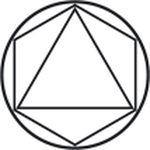
\includegraphics{TUMlMschwarz.png}\\[15mm]

Bachelor's Thesis\\[15mm]

{\Huge
  The 27 Lines on a Cubic Surface
}
\bigskip

\normalsize

Long Huynh Huu <long.huynh-huu@tum.de>
\end{center}
\vspace*{75mm}

Supervisor: Christian Liedtke <liedtke@ma.tum.de>
\medskip

Advisor: Christian Liedtke <liedtke@ma.tum.de>
\medskip

Submission Date: October 27th, 2014

\end{titlepage}

%%%% The following has to be signed by hand!

\vspace*{150mm}

I assure the single handed composition of this bachelor's thesis only supported by declared resources.
\bigskip

Garching, 
\newpage


\section*{Zusammenfassung}
%TODO: Auf Deutsch
xxxxxxxxxxxx deutsche Zusammenfassung xxxxxxxxxx

In this Bachelor thesis I will prove in full detail the existence of 27 lines on an arbitrary smooth cubic in projective $n$-space over an algebraically closed field $k$.

\newpage
\tableofcontents
\newpage

\pagenumbering{arabic}
\pagestyle{headings}


% \section{Change of coordinates}

\subsection{Notes to myself}

In this section I introduce definitions and hands-on examples to work with geometric objects in the language of scheme theory, or maybe I'll just drop the generalities and work with elementary algebra.
Particular goals are
\begin{itemize}
\item the definition of what a change of coordinates means precisely and work out the details to use it without regret in the proof of the main result.
\item the definition of what it means for a variety to contain a doubled line. In scheme theoretic language it is as simple as saying, that this variety has a subscheme isomorphic to a doubled line! Again, I might drop the notion of schemes, or work with it.
\end{itemize}
So this text also aims to be educational and close the gap between the intuitive and the technical.

It might be interesting to
\begin{itemize}
\item introduce the category of varieties and rational functions. \textbf{If needed}.
\end{itemize}

\subsection{Affine linear transformations of affine space}

An important notion which will appear again and again is the change of coordinates.
In affine space one thinks of a linear transformation $T:\affine^n_k \to \affine^n_k$.
Now observe the effect of such a transformation on a hypersurface $V(I)$, $I = (f)$:
$ T(V(I)) = \{ Tx \in k^n: f(x) = 0 \} = \{y \in k^n : f(T^{-1}y) = 0\}$
So one may define a linear transformation on a variety by precomposing the inverse to the polynomial functions.
But let me suggest a different definition of linear transformation which does not necessarily require $T$ to be invertible and which is compatible with the scheme theoretic notion of a morphism.

\begin{definition} Let $A = (a_{ij}) \in M(n,k)$ be a $n\times n$-matrix. Then we can define a homomorphism of polynomial rings
\begin{align}
T^\#_A : k[X_1,.. X_n] &\to k[X_1,.. X_n], \\
X_i &\to \sum_{j=1}^n a_{ij}X_j.
\end{align}
\end{definition}

This induces a morphism $T_A : \affine^n_k \to \affine^n_k$ of affine schemes. Indeed, this definition does what we expect.

\begin{proposition} By Hilbert's Nullstellensatz a point $(x_1,..x_n) \in k^n$ corresponds to a maximal ideal $(X_1-x_1,.. X_n-x_n) \subset k[X_1,..X_n]$.
$T_A$ maps the subscheme $V(X_1-x_1,..X_n-x_n)$ to $V(X_1-y_1,..X_n-y_n)$ where $(y_1,..y_n) = A(x_1,..x_n)$.
\end{proposition}

\begin{proof} If $A$ is invertible, we basically apply the Gauß-Jordan algorithm....
\end{proof}

Don't forget the translations: $X_i \mapsto X_i + t_i$.
Together we get affine linear transformations.


\subsection{Rational maps}

Fancy category language here...

\section{General facts}

\subsection{projective space}

In order to do geometry we need to explain what points, lines, surfaces are, and this can be done in several ways, synthetically or analytically.

There are several formulations of projective space, with varying degree of generality, and for our purposes I have chosen the one in terms of homogeneous coordinates.

Let $k$ be an algebraically closed field and $n$ a natural number.
The projective space $\proj^n_k$ is a topological space given as set by  $k^{n+1} - \{ 0 \}$ modulo the relation $X=(x_0,..x_n) \sim Y=(y_0,..y_n)$ if and only if $X$ and $Y$ are linearly dependent (as vectors in $k^{n+1}$). The equivalence class of $X$ will be denoted $[x_0:x_1:..:x_n]$.

The topology is given by the closed subsets
\begin{equation}
\V(I) =
\mkset{ [x_0:..x_n] \in \proj^n_k}
      { \forall f\in I \text{ homogeneous}, f(x_0,..x_n) = 0}
\end{equation}
for homogeneous ideals $I$ of the polynomial ring $k[x_0,..x_n]$.
The topology is known as Zariski's topology.
Because $k[x_0,..x_n]$ is a Noetherian ring, every ideal is finitely generated and in particular every homogeneous ideal is finitely generated by homogeneous elements.
So we may say that a closed set consists precisely of the points in projective space where a finite set of homogeneous ideals vanish.

In this framework I want to identify geometric objects with homogeneous ideals of $k[x_0,..x_n]$.
However, most of the time it is easier to speak of the closed subsets of projective space, instead of the ideal $I$, and $I$ itself can be recovered by means of Hilberts's Nullstellensatz in the form of its radical.

A \emph{hypersurface} is given by one equation $f=0$ for $f\in k[x_0,..x_n]$, and its set of points is $\V(f)$.
In case of $f$ being a linear form we call $\V(f)$ a \emph{hyperplane}.

A line is determined by $n-1$ $k$-linearly independent linear forms and a point by $n$ $k$-linearly independent linear forms.



\subsubsection{linear sets}
\begin{todo}
\item define hyperplane, plane, line, point
\item closed subsets yield reduced ideals, but we may attach non-reduced ideals. brought to its full conclusion, we need schemes, but we can do without so far
\item MOVED FROM CONIC SECTION: Of course, in the projective plane there always exists an intersection for any two lines.
% TODO: move this to the front
(This is just a consequence of linear algebra: Say $h_1 = a_0x_0 + a_1x_1 + a_2x_2, h_2 = b_0x_0 + b_1x_1 + b_2x_2$, then the kernel of the matrix $\begin{pmatrix} a_0 & a_1 & a_2 \\ b_0 & b_1 & b_2 \end{pmatrix}$ is nontrivial and if $(s_0,s_1,s_2) \neq 0 \in k^3$ lies in the kernel, then $P := [s_0:s_1:s_2]$ lies in the intersection.)


\end{todo}

\subsubsection{Hilbert's Nullstellensatz}

\begin{todo}
\item put the projective nullstellensatz here
\item corollary for radical $f$: $\V(f) \subset \V(f_0,..f_r) \implies \sqrt{(f_0,..fr)} \subset \sqrt{(f)} \implies f \text{ divides all } f_i$
\item in ptic. if $f$ is a 1-form or a non-singular cubic (as to be seen later)
\end{todo}

\subsection{partial derivatives}

In this section we discuss partial derivatives -- a useful algebraic tool to obtain some geometric properties.
 % TODO

\begin{definition}[partial derivative]
Let $D : k[x_0,..x_n] \to k[x_0,..x_n]$ be a derivation over $k$, i.e. a homomorphism of $k$-modules which satisfies the Leibniz rule $D(xy) = xDy+yDx$ for $x,y \in k[x_0,..x_n]$. Furthermore let $D(h) \in k$ for every linear form $h$. We call such a derivation a \emph{partial derivative}.
\end{definition}

\begin{example}
The standard example for partial derivatives are of course the partial derivates with respect to one of the variables $x_i$, defined as $\del_{x_i}(x_j) = \delta_{i,j} := \begin{cases} 1, & \text{ for } i = j \\ 0, & \text {otherwise.} \end{cases}$
\end{example}

\begin{example}
For any monomial $\{ h_i\}_{i=0}^n$ basis of $\bigoplus_{i=0}^n kx_i \subset k[x_0,..x_n]$ we obtain a family of partial derivatives $\{ \del_{h_i} \}_{i=0}^n$ for which $\del_{h_i}(h_j) = \delta_{i,j}$ holds. The construction goes as follows: Let $M = (a_{i,j})  \in k^{(n+1)\times(n+1)}$ be the base change matrix and $M^{-1} = (\widetilde a_{i,j})$ be its inverse.
This just means $h_i = \sum_{j=0}^n a_{i,j} x_j$ and hence $\del_{x_k}(h_i) = a_{i,k}$.
From $\delta_{i,j} = \sum_{k=0}^n a_{i,k}\widetilde a_{k,j}
= \sum_{k=0}^n \del_{x_k}(h_i) \widetilde a_{k,j}$ it is obvious that we need to define

\begin{equation}
\del_{h_j} = \sum_{k=0}^n \widetilde a_{k,j} \del_{x_k}
\end{equation}

Another way to write this would be
\begin{equation}
\begin{pmatrix} \del_{h_0} \\ \vdots \\ \del_{h_n} \end{pmatrix}
= M^{-T}
\begin{pmatrix} \del_{x_0} \\ \vdots \\ \del_{x_n} \end{pmatrix}
\end{equation}
\end{example}

A useful fact, that allows us to recover a homogeneous polynomial by its partial derivatives is

\begin{proposition}[Euler's formula]
For any $f \in k[x_0,..x_n]$ homogeneous of degree $d$ we have the equality
\[ df = \sum_{i=0}^n \del_{x_i}(f)x_i \]
\end{proposition}
\begin{proof}
By linearity we only need to prove the monomial case $f = \prod_{i=0}^n x_i^{a_i}$, $a_i$ being integers such that $\sum_{i=0}^n a_i = d$.
\begin{equation}
\sum_{i=0}^n \del_{x_i}(f)x_i
= \sum_{i=0}^n \begin{Bmatrix} \left(\prod_{j\neq i} x_j^{a_j}\right) a_i x_i^{a_i-1} x_i, & \text{ for } a_i > 0
\\ 0, &\text{ for } a_i = 0 \end{Bmatrix}
= \sum_{i=0}^n a_i f = df
\end{equation}
\end{proof}

\begin{corollary}
$\V(\del_{x_0}(f),..\del_{x_n}(f), df) = \V(\del_{x_0}(f),..\del_{x_n}(f))$
\end{corollary}


\begin{lemma}
Let $\del_1,\del_2$ be partial derivatives, then $\del_1.\del_2 = \del_2.\del_1$.
\end{lemma}
\begin{proof}
We only need to prove this for monomials, and we'll perform an induction on the degree.
If $f$ is a monomial of degree less than 2, then $\del_1(\del_2(f)) = 0 = \del_2(\del_1(f))$. 
Now suppose $f = x_if'$ and $\del_1(\del_2(f')) = \del_2(\del_1(f'))$.

\begin{equation}
\del_1.\del_2(x_if') = \del_1(x\del_2(f') + f'\del_2(x)) = 
\del_1(x)\del_2(f') + \del_1(f')\del_2(x) + x\del_1(\del_2(f')) + \underset{=0}{\underbrace{f'\del_1(\del_2(x))}}
\end{equation}
The last term is symmetric in $\del_1,\del_2$ (by assumption).
\end{proof}

\begin{corollary}[Taylor's formula]
Let $f \in k[x_0,..x_n]$ be a polynomial and $f = \sum_{i=0}^d f_i$ its decomposition into homogeneous parts.
Then $f_i = \frac{1}{i!} \sum_{|\bf{\alpha}|=i} \del^{\bf{\alpha}}(f)(0)x^{\bf{\alpha}}$ in multi-index notation.
\end{corollary}
\begin{proof}
% TODO ...
\end{proof}



\subsection{Singularities and the tangent space}

In this section we want to study the local properties of a projective variety.
A particularly simple tool is the tangent space.
The analytical idea behind it is to approximate, say, a surface near a point by a plane as close as possible.
That's what a Frechét differential does for, say,  the graph of some differentiable function $\reals^2 \to \reals$.
In the analytical world such a plane is defined via partial derivatives, which can be emulated for polynomials in a purely algebraic way.

\subsubsection{Partial derivatives}
\begin{definition}
Let $D : k[x_0,..x_n] \to k[x_0,..x_n]$ be a \emph{derivation} over $k$, i.e. a homomorphism of $k$-modules which satisfies the Leibniz rule $D(xy) = xDy+yDx$ for $x,y \in k[x_0,..x_n]$. Furthermore let $D(h) \in k$ for every linear form $h$. We call such a derivation a \emph{partial derivative}.
\end{definition}

\begin{example}
The standard example for partial derivatives are of course the partial derivatives with respect to one of the variables $x_i$, defined as $\del_{x_i}(x_j) = \delta_{i,j} := \begin{cases} 1, & \text{ for } i = j \\ 0, & \text {otherwise.} \end{cases}$
\end{example}

\begin{example} \label{exampleAlternativePartialDerivatives}
For any basis $\{ h_i\}_{i=0}^n$ of the vector space of linear forms $\bigoplus_{i=0}^n kx_i \subset k[x_0,..x_n]$ we obtain a family of partial derivatives $\{ \del_{h_i} \}_{i=0}^n$ for which $\del_{h_i}(h_j) = \delta_{i,j}$ holds. The construction goes as follows: Let $M = (a_{i,j})  \in k^{(n+1)\times(n+1)}$ be the base change matrix and $M^{-1} = (\widetilde a_{i,j})$ be its inverse.
This just means $h_i = \sum_{j=0}^n a_{i,j} x_j$ and hence $\del_{x_k}(h_i) = a_{i,k}$.
From $\delta_{i,j} = \sum_{k=0}^n a_{i,k}\widetilde a_{k,j}
= \sum_{k=0}^n \del_{x_k}(h_i) \widetilde a_{k,j}$ it is obvious that we need to define

\begin{equation}
\del_{h_j} = \sum_{k=0}^n \widetilde a_{k,j} \del_{x_k}
\end{equation}

Another way to write this would be
\begin{equation}
\begin{pmatrix} \del_{h_0} \\ \vdots \\ \del_{h_n} \end{pmatrix}
= M^{-T}
\begin{pmatrix} \del_{x_0} \\ \vdots \\ \del_{x_n} \end{pmatrix}
\end{equation}
\end{example}

A useful fact, that allows us to recover a homogeneous polynomial by its partial derivatives is

\begin{proposition}[Euler's formula]
For any $f \in k[x_0,..x_n]$ homogeneous of degree $d$ we have the equality
\[ d\cdot f = \sum_{i=0}^n \del_{x_i}(f)x_i \]
\end{proposition}
\begin{proof}
By linearity we only need to prove the monomial case $f = \prod_{i=0}^n x_i^{a_i}$, $a_i$ being integers such that $\sum_{i=0}^n a_i = d$.
\begin{equation}
\sum_{i=0}^n \del_{x_i}(f)x_i
= \sum_{i=0}^n \begin{Bmatrix} \left(\prod_{j\neq i} x_j^{a_j}\right) a_i x_i^{a_i-1} x_i, & \text{ for } a_i > 0
\\ 0, &\text{ for } a_i = 0 \end{Bmatrix}
= \sum_{i=0}^n a_i f = df
\end{equation}
\end{proof}

\begin{corollary}
$\V(\del_{x_0}(f),..\del_{x_n}(f), df) = \V(\del_{x_0}(f),..\del_{x_n}(f))$
\end{corollary}

\begin{lemma} \label{lemmaPartialDerivativesCommute}
Let $\del,\del'$ be partial derivatives, then $\del.\del' = \del'.\del$.
\end{lemma}
\begin{proof}
We only need to prove this for monomials, and we'll perform an induction on the degree.
If $f$ is a monomial of degree less than 2, then $\del(\del'(f)) = 0 = \del'(\del(f))$. 
Now suppose $f = x_if'$ and $\del(\del'(f')) = \del'(\del(f'))$.

\begin{equation}
\del.\del'(x_if') = \del\left(x_i\del'(f') + f'\del'(x_i)\right) = 
\del(x_i)\del'(f') + \del(f')\del'(x_i) + x_i\del(\del'(f')) + f'\underset{=0}{\underbrace{\del(\del'(x_i))}}
\end{equation}
The last term is symmetric in $\del,\del'$ (by induction hypothesis).
\end{proof}

As a final fact about partial derivatives, I want to state the chain rule.
\begin{lemma}[chain rule]
Let $f \in k[x_0,..x_n]$ be a homogeneous polynomial and $F_0,..F_n \in k[x_0,..x_m]$ homogeneous polynomials of same degree.
They define a morphism $F : \proj^m_k \to \proj^n_k$.
We define the composition $f.F := f(F_0,..F_n)$.
Then, the following equality holds for $0 \leq i \leq n$:
\begin{equation}
\del_{x_i} (f.F) = \sum_{j=0}^n ((\del_{x_j}f).F) \cdot \del_{x_i}(F_j)
\end{equation}
\end{lemma}
We just give a proof sketch: Verify the equation for $f$ being a power of one variable, then for $f$ being a monomial and finally for a general polynomial $f$. \hfill\qedsymbol

The following formula will come in handy for some calculations.
It will allow us to understand terms of the form $f(P+Q)$ for a homogeneous polynomial $f$ and points $P,Q$ better.
The idea is kind of related to Taylor's formula, which allows one to understand terms of the form $f(x + \delta)$.
\begin{proposition}[poor student's Taylor expansion] \label{propositionTaylor}
Let $f \in k[x_0,..x_n]$ be a homogeneous polynomial of degree $d$.
There exists a unique decomposition of $f(X+X') := f(x_0+x'_0,..x_n+x'_n) \in k[x_0,..x_n,x'_0,..x'_n], \quad X := (x_0,..x_n), X' := (x'_0,..x'_n)$ into the sum
\begin{equation}
f = \sum_{i=0}^d f^{(i)}
\end{equation}
where $f^{(i)}$ is homogeneous of degree $i$ in the variables $x'_0,..x'_n$ and homogeneous of degree $d-i$ in the variables $x_0,..x_n$.

The $f^{(i)}$ are symmetric in the sense that $f^{(i)}(X;X') = f^{(d-i)}(X';X)$ for $1 \leq i \leq d$.
For $i = 0,1$ we have the explicit formulas
\begin{align}
f^{(0)}(X;X') =& f(X)  \label{eqPolar1}
\\ f^{(1)}(X;X') =& \sum_{i=0}^n (\del_{x_i}f)(X) x'_i \label{eqPolar2}
\end{align}
\end{proposition}
\begin{proof}
The polynomial $f(X+X')$ is homogeneous in $k[x_0,..x_n;x'_0,..x'_n]$ with the standard grading.
The existence of the decomposition and its uniqueness follow immediately by considering $f(X+X')$ as element of, say, $k(x_0,..x_n)[x'_0,..x'_n]$.
The symmetry property comes by applying the decomposition to $f(X'+X)$ (just interchange $X$ and $X'$), but obviously $f(X'+X) = f(X+X')$.
By comparing degrees in the variables $x_0,..x_n$ we then get $f^{(i)}(X;X') = f^{(d-i)}(X';X)$ as desired.
Equation \ref{eqPolar1} holds, as $f(X+0) = \sum_{i=0}^d f^{(i)}(X;0,..) = f^{(0)}(X;0)$.
We can see that equation \ref{eqPolar2} holds too:
We can isolate the degree 1 terms in $x'_0,..x'_n$ by taking the partial derivatives and evaluating at $X'=0$.
This forgets the terms of degree 0 and degree $\geq 2$.
Then we can recover $f^{(1)}$ by Euler's formula.
Hence $f^{(1)}(X;X') = \sum_{i=0}^n (\del_{x'_i}f(X+X'))(X;0,..) x'_i
\overset{\text{chain rule}}= \sum_{i=0}^n \left( \sum_{j=0} \del_{x'_j}f(X+X') \del_{x'_i}(x_j + x'_j) \right)(X;0,..)x'_i = \sum_{i=0}^n (\del_{x'_i} f)(X) x'_i$.
\end{proof}

\begin{remark}
The polynomial $f^{(1)}$ is also called the \emph{polar form} of $f$ in \cite[p. 104]{reid1988undergraduate}.
\end{remark}

\begin{corollary} \label{corollaryTaylorForQuadricAndCubic}
Let $g$ be a quadratic form and $f$ a cubic form. Then
\begin{align}
g(X+X') =& g(X) + g^{(1)}(X;X') + g(X')
\\ f(X+X') =& f(X) + f^{(1)}(X;X') + f^{(1)}(X';X) + f(X')
\end{align}
In particular, for $X=X'$: $4g(X) = g(X+X) = g(X) + g^{(1)}(X;X) + g(X)$ so $2g(X) = g^{(1)}(X;X)$ or conversely $g^{(1)}(X;X') = g(X+X') - g(X) - g(X')$, so we may view $g^{(1)}(X;X')$ as symmetric bilinear form.
\end{corollary}

\begin{example}
Let's say $f = x^3 + y^3 - xyz \in k[x,y,z]$ and we want to understand $f(x+d_x,y+d_y,z+d_z) \in k[x,y,z,t,d_x,d_y,d_z,d_t]$.
This yields
\begin{align*}
f(x+d_x,y+d_y,z+d_z)
  =& (x^3 + y^3 - xyz)
\\+& (3x^3d_x + 3y^2d_y + yzd_x + xzd_y + xyd_z)
\\+& (3d_x^3x + 3d_y^2y + d_yd_zx + d_xd_zy+d_xd_yz)
\\+& (d_x^3 + d_y^3 - d_xd_yd_z)
\end{align*}
\end{example}


\subsubsection{The tangent space}

\begin{definition} \label{definitionTangentSpace}
Let $I \subset k[x_0,..x_n]$ be a homogeneous ideal, $\V(I)$ a projective variety in $\proj^n_k$ and $P\in \V(I)$ a point on that variety.
If $I$ is generated by a single homogeneous polynomial $f$, then we define $T_P(\V(f))$ to be the variety $\V(f^{(1)}(P))$ where $f^{(1)}(P) := f^{(1)}(P;x_0,..x_n)$.
If $I$ is generated by homogeneous polynomials $f_0,..f_r$, then we define $T_P(\V(I)) = \bigcap_{i=0}^r T_P(f_i)$.
We will see in a second that the choice of generators does not matter.
\end{definition}

\begin{example} \label{exampleTangentPlaneOfLinearSubsets}
Let's consider some trivial examples first.
The tangent space of a hyperplane $\V(h)$ at any point $P$ is the hyperplane itself, by Euler's formula:
\begin{equation}
h = \sum_{i=0}^n \underset{\in k}{\underbrace{(\del_{x_i}h)}}x_i = \sum_{i=0}^n (\del_{x_i}h)(P) x_i = h^{(1)}(P)
\end{equation}
The same holds for \emph{linear subspaces}, which are just intersections of hyperplanes (for instance lines or points).
\end{example}

\begin{example}
Suppose $I \subset J \subset k[x_0,..x_n]$ are homogeneous ideals, $P \in \V(I)$.
One can see that $T_P(I) \subset T_P(J)$ as follows: Let $f_0,..f_r$ be generators of $I$ and $g_0,..g_s$ be generators of $J$.
Because $I$ lies in $J$, we can write each $f_i$ as sums of products of the $g_j$.
By definition $T_P(\V(J)) = \bigcap_{j=0}^s \V(g_j^{(1)})$.
Consider now the set $K = \mkset{ f \in k[x_0,..x_n] }{f^{(1)}(P) \text{ vanishes on }T_P(\V(J))}$.
By the identities $(f+g)^{(1)}(P) = f^{(1)}(P) + g^{(1)}(P)$ and $(fg)^{(1)}(P) = f(P)g^{(1)}(P) + g(P)f^{(1)}(P)$ it can be easily checked that $K$ is an ideal.
Because it contains the $g_j$, it also contains the $f_i$.
This shows that $\V(J) \subset \V(I)$ implies $T_P(\V(J)) \subset T_P(\V(I))$ and hence by choosing $I=J$ it also shows that the choice of generators in Definition \ref{definitionTangentSpace} did indeed not matter.
\end{example}

\begin{example}
Consider the family of cubic curves in $\proj^2_k$ given by $y^2z - x^3 - axz^2 \in k[x,y,z]$, $a \in k$ and let $P = [0:0:1] \in \V(y^2z - x^3 - axz^2)$.
The equation of the tangent space is $ax$, hence the tangent space is the line $x = 0$ unless $a = 0$ in which case the tangent space is the whole $\proj^2_k$.
Points for which the tangent space `degenerates' are rather special and hence deserve a name.
\end{example}


\begin{definition}
A \emph{singular} point of a hypersurface $\V(f) \subset \proj^n_k$ is a point in $\V(f,\del_{x_0}f,..\del_{x_n}f)$.
In other words, a point $P$ is singular iff $T_P(\V(f)) = \proj^n_k$.
\end{definition}

Singular points are worth studying because they behave well under automorphisms of projective space.

\begin{proposition} \label{propositionTangentTransform}
Let $\phi : \proj^n_k \to \proj^n_k$ be a projective transformation.
Then $\phi(T_P(\V(f))) = T_{\phi(P)}(\phi(\V(f)))$.
\end{proposition}

This is actually a corollary of a more general fact about \emph{linear embeddings}.

\begin{proposition} \label{corollaryTangentPullback}
Let $V\subset \proj^N_k$ be a subvariety, $\iota = (\iota_0,..\iota_N): \proj^n_k \hookr \proj^N_k$ a linear embedding and $\iota^{-1}(V) \subset \proj^n_k$.
Thus, we have a commutative diagram:
\begin{equation}
\begin{xy}
(0,20)*+{\proj^n_k}="pn";
(30,20)*+{\proj^N_k}="pN";
(0,0)*+{\iota^{-1}(V)}="iv";
(30,0)*+{V}="v";
{\ar@{^{(}->} "pn";"pN"}?*!/_2mm/{\iota};
{\ar@{^{(}->} "iv";"v"}?*!/_2mm/{\iota|_{\iota^{-1}(V)}};
{\ar@{_{(}->} "iv";"pn"};
{\ar@{_{(}->} "v";"pN"};
\end{xy}
\end{equation}
Then $T_{\iota^{-1}(P)}(\iota^{-1}(V)) = \iota^{-1}(T_P(V)) $ holds for $P$ in the image of $\iota$.
\end{proposition}
\begin{proof}
Because intersections are well-behaved under preimages, we may assume $V$ to be a hypersurface, say $\V(f)$.
We have the equalities $\iota^{-1}(T_P(\V(f))) = \iota^{-1}(\V(f^{(1)}(P))) = \V(f^{(1)}(P).\iota)$ and $T_{\iota^{-1}(P)}(\iota^{-1}(\V(f))) = T_{\iota^{-1}(P)}(\V(f.\iota)) = \V((f.\iota)^{(1)}(\iota^{-1}(P)))$, therefore it's enough to show
\begin{equation}
(f.\iota)^{(1)}(\iota^{-1}(P))
=
f^{(1)}(P).\iota
\end{equation}

The calculation goes as follows
\begin{align}
(f.\iota)^{(1)}(\iota^{-1}(P))
  \defeq& \sum_{i=0}^n \del_{x_i}(f.\iota)(\iota^{-1}(P))x_i
\\\overset{\text{chain rule}}=& \sum_{i=0}^n \left(\sum_{j=0}^n ((\del_{x_j}f).\iota) \cdot \underset{\in k}{\underbrace{\del_{x_i}(\iota_j)}}\right)(\iota^{-1}(P))x_i
\\\overset{\text{evaluate at }\iota^{-1}(P)}=& \sum_{i=0}^n \left(\sum_{j=0}^n (\del_{x_j}f)(P) \cdot \del_{x_i}(\iota_j)\right)x_i
\\\overset{\text{interchange summation}}=& \sum_{j=0}^n (\del_{x_j}f)(P) \sum_{i=0}^n \del_{x_i}(\iota_j))x_i
\\\overset{\text{Euler's formula}}=& \sum_{j=0}^n (\del_{x_j}f)(P) \iota_j
\\\defeq& f^{(1)}(P).\iota
\end{align}
\end{proof}

\begin{corollary}
Let $\phi : \proj^n_k \to \proj^n_k$ be a projective transformation and $S = \V(f)$ a hypersurface.
Then a point $P \in S$ is singular iff $\phi(P) \in \phi(S)$ is.
\end{corollary}
\begin{proof}
The hypersurface $S$ is singular at $P$ iff $T_P(S) = \proj^n_k$ iff $T_{\phi(P)}(\phi(S)) = \phi(T_P(S)) = \proj^n_k$ iff $\phi(S)$ is singular at $\phi(P)$.
\end{proof}

\begin{corollary} \label{corollaryIntersectionWithTangent}
Let $S = \V(I) \subset \proj^N_k$ be a projective variety, $P\in S$.
Clearly, as intersection of hyperplanes the tangent space at $P$ is a linear subspace of $\proj^N_k$ and hence the image of some linear embedding $\iota : \proj^n_k \hookr \proj^N_k$.
$\iota^{-1}(S)$ has a singularity at $\iota^{-1}(P)$.
\end{corollary}
\begin{proof}
By corollary \ref{corollaryTangentPullback} the tangent space of $\iota^{-1}(S)$ at $\iota^{-1}(P)$ is $\iota^{-1}(T_P(S)) = \iota^{-1}(\var{im}(\iota)) = \proj^n_k$, thus $\iota^{-1}(P)$ is a singular point.
\end{proof}

\subsection{Plane conics and conic surfaces}

\subsubsection{The question of degeneracy}

A plane conic is a algebraic variety $\V(g)$ given by a quadratic form $g \in k[x_0,x_1,x_2]$. One might ask the question whether the conic is a union of two lines (in which case the conic is called \emph{degenerate}), or in algebraic terms, whether $g$ factors into two linear forms or whether it is irreducible.
Let's turn our attention the an easier question: When is a conic singular?

Assume that the characteristic of our base field $k$ is not 2, then the conic can be written, for appropriate coefficients $a,b,c,d,e,f \in k$ as:
\begin{equation}
g = ax_0^2 + bx_0x_1 + cx_1^2 + dx_0x_2 + ex_1x_2 + fx_2^2
\end{equation}
The singular points are given by the system of equations
\begin{equation}
\del_{x_0} g = \del_{x_1} g = \del_{x_2} g = 0
\end{equation}
which written out in matrix notation, amounts to
\begin{align}
\underset{=:M}{\underbrace{
\begin{pmatrix}
2a & b & d \\
b & 2c & e \\
d & e & 2f
\end{pmatrix}
}}
\begin{pmatrix}
x_0 \\ x_1 \\ x_2
\end{pmatrix}
= 0
\end{align}
We call the matrix $M$.
A singular point $[s_0:s_1:s_2] \in \proj^2_k$ would of course be a non-zero solution of above equation and as such can only exist precisely if the determinant of $M$ vanishes.
So far we have obtained

\begin{corollary}
Let $k$ be a field of characteristic not 2 and $g =  ax_0^2 + bx_0x_1 + cx_1^2 + dx_0x_2 + ex_1x_2 + fx_2^2
\in k[x_0,x_1,x_2]$ be a quadratic form. The conic $\V(g) \subset \proj^2_k$ is singular if and only if
\begin{equation}
\frac 12
\det
\begin{pmatrix}
2a & b & d \\
b & 2c & e \\
d & e & 2f
\end{pmatrix}
= 4acf + bde - ae^2 - cd^2 - fb^2
\end{equation}
\end{corollary}

Incidentally this statement holds true for characteristic 2 as well, even though we need to approach the proof a little differently.
At this point I remind the reader that addition and subtraction are the same in characteristic 2, in the sense that negation operation is just the identity, which will simplify the calculations a little.
The corollary then translates to $g$ having a singular point if and only if $bde +ae^2 + cd^2 +fb^2 = 0$.
The set of singular points is by definition the intersection of $V = \V(\del_{x_0}g,\del_{x_1}g,\del_{x_2}g)$ and $\V(g)$, so let's calculate the points in the first variety: Assuming that not all coefficients $b,d,e$ vanish, the only point on $V$ is $[e:d:b]$, as can be seen by Gaussian elimination where we distinguish the cases of $0,1$ or $2$ of the coefficients $b,d,e$ vanishing.
This point $[e:d:b]$ lies on $\V(g)$ iff $0 = g(e,d,b) = ae^2 + bde + cd^2 + dbe + ebd + fb^2 = bde + ae^2 + cd^2 + fb^2$ as desired.
If all of $b,d,e$ vanish, then $V$ is the whole space and every point of $\V(g)$ is singular ($\V(g) = \V((\sqrt{a}x_0 + \sqrt{c}x_1 + \sqrt{f}x_2)^2)$ being a doubled line) and also $bde + ae^2 + cd^2 + fb^2 = 0$. We have proven:

\begin{corollary} \label{corollarySingularConic}
Let $k$ be a field of any characteristic and $g = ax_0^2 + bx_0x_1 + cx_1^2 + dx_0x_2 + ex_1x_2 + fx_2^2
 \in k[x_0,x_1,x_2]$ be a quadratic form. The conic $\V(g) \subset \proj^2_k$ is singular if and only if $4acf + bde - ae^2 - cd^2 - b^2f = 0$.
\end{corollary}


Returning to our initial question we want to establish the fact that the conic given by the quadratic form $g$ is irreducible if and only if it is nonsingular.
For that assume reducibility, that is $g = h_1h_2$ for 1-forms $h_1$ and $h_2$.
We can apply the following lemma
\begin{lemma} \label{lemmaSingularIntersect}
Let $\V(I),\V(J)$ be two varieties. Then the union of $\V(IJ)$ is singular at their intersection $\V(I,J)$.
\end{lemma}
\begin{proof}
Let $f\in I, g\in J$, $P\in \V(I,J)$. We get $(fg)^{(1)}(P) = f(P)g^{(1)}(P) + g(P)f^{(1)}(P) = 0$, hence the tangent space at $P$ is the whole space.
\end{proof}
It says that the intersection of the two lines $\V(h_1)$ and $\V(h_2)$ (and we've seen that lines in $\proj^2_k$ do indeed intersect) is a singular point of our conic.

The converse can be seen as follows. Let $P=[p_0:p_1:p_2]$ be a singularity and $P'=[p'_0:p'_1:p'_2]$ is any other point on the conic (for instance any intersection point of $\V(g) \cap \V(x_i)$, $i$ such that $p_i \neq 0$).
For $g$ to be singular at $P$ means in particular that $g^{(1)}(P,P') = \sum_{i=0}^2 \del_{x_i}g(P)p'_i = 0$ using proposition \ref{propositionTaylor}.
By corollary \ref{corollaryTaylorForQuadricAndCubic}, we can expand $g(\lambda P + \mu P') = \lambda^2 g(P) + \lambda\mu g^{(1)}(P;P') + \mu^2 g(P')= 0$.
Hence $g$ vanishes on the line $\overline{P,P'}$ and Hilbert's Nullstellensatz implies that the conic is a union of two lines.

\begin{theorem}
Let $k$ be a field and $\V(g) \subset \proj^2_k$ a conic given by a quadratic form $g = ax_0^2 + bx_0x_1 + cx_1^2 + dx_0x_2 + ex_1x_2 + fx_2^2$.
Then the following are equivalent:
\begin{enumerate}
\item The conic is degenerate.
\item The quadratic form $g$ factors into two linear forms, $g=h_1h_2$.
\item The conic is singular.
\item $4acf + bde - ce^2 - ad^2 - b^2f = 0$
\end{enumerate}
\end{theorem}


\begin{remark}
Otto Hesse has shown that over $k=\complex$ a curve $\V(g)$ decomposes into lines iff the Hessian curve $\V(\det(\del_{x_i}\del_{x_j}h))$ lies in $\V(g)$ (\cite[p.289]{brieskorn2012plane}), however we've seen that this result does not hold over arbitrary fields.
The equation of the Hessian curve in case of the conic considered in this section is precisely $2(4acf + bde - ce^2 - ad^2 - b^2f) = 0$.
\end{remark}


\subsubsection{The two rulings of a nonsingular quadric surface}


It is now time to profit from the previous meditations about singularities.
Let $Q \subset \proj^3_k$ be a nonsingular quadric surface.
We will see that it does not make sense to count the lines on this surface, but let's find some first.
Surely $Q$ will not contain any plane, as this would mean (appealing to the Nullstellensatz) that $Q$ is the union of two planes.
Furthermore these planes intersect at least in a line, so by lemma \ref{lemmaSingularIntersect} the quadric surface would be singular.
As a first step, choose a point $P \in Q$.
Because $Q$ does not contain planes, the tangent space intersects $Q$ in a conic curve.
This curve is singular at $P$ by lemma \ref{lemmaIntersectionWithTangent}, therefore it is the union of two lines $L_1,L_2$.

Each $L_i$ gives a family of lines as follows: For a point $P'$ on $L_i$, we may intersect again $Q$ with $T_{P'}Q$.
Here too we obtain the union of two lines, one of which being $L_i$, the other line we call $L_i(P')$.
By this definition $L_1(P) = L_2$ and $L_2(P) = L_1$.
We say that the family $\mathcal F(L_i) := \mkset{ L_i(P') }{P' \in L_i}$ is the \emph{family generated by $L_i$}.

In fact, these are all the lines on $Q$, which is obvious from the following consideration.
Let $Z$ be any line on $Q$ which is neither $L_1$ nor $L_2$, then it intersects the plane $T_P(Q)$ in one point (corollary \ref{corollarySimpleIntersect}).
This point lies precisely on one of the two $L_i$ (suppose that was not the case, then $P \in Z \subset Q \implies Z = T_P(Z) \subset T_P(Q) \implies Z=L_1 \text{ or } Z=L_2$) so $Z = L_i(T_P(Q)\cap Z)$.
Conversely note, that we have chosen $P$ arbitrarily, so any point of $Q$ is the intersection of two lines $M_1,M_2$ on $Q$ and each of the two lines belong to the family generated by $L_1$ or $L_2$.
It, however, cannot occur that both lines belong to the same family, say parametrised by $L_1$. In that case, $M_1,M_2,L_1$ would lie on the same tangent plane, but $Q$ intersects a tangent plane in just two lines!
We can conclude therefore:
\begin{proposition}
There are two families $\mathcal F(L_1), \mathcal F(L_2)$ of lines on $Q$ and each line on $Q$ belongs to just one family.
The lines in each family are disjoint and as set the union of any one family covers all of $Q$.
\end{proposition}
A little bit more can be said.
Consider a line $L' \in \mathcal F(L_1)$.
Because $L_1 \in \mathcal F(L')$ and $L_1 \in \mathcal F(L_2)$, the family generated by $L'$ must be $\mathcal F(L_2)$ by previous proposition, but this just means that $L'$ intersects all the lines in $\mathcal F(L_2)$!
Hence we deduced
\begin{corollary} \label{corollaryMutualIntersect}
Any line in $\mathcal F(L_1)$ intersects any other line in $\mathcal F(L_2)$.
\end{corollary}

\begin{figure}
\center
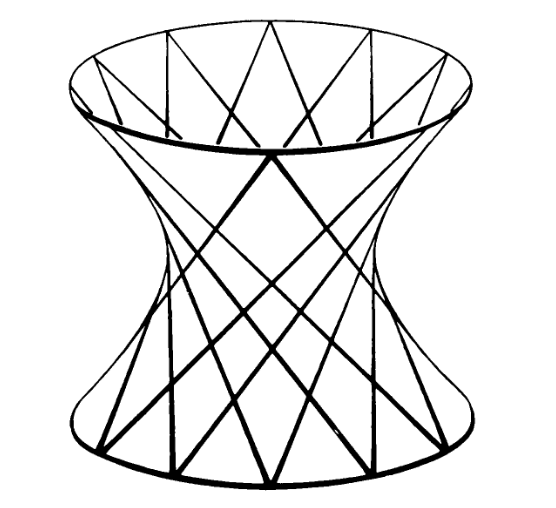
\includegraphics[width=.4\textwidth]{img/ruledsurface-hilbert.png}
\caption{An illustration of the rulings on the quadric surface `Anschauliche Geometrie' by Hilbert and Cohn-Vossen \cite[figure 17]{cohn1990geometry}}
\end{figure}

\begin{remark}
Over an algebraically closed field, a line has infinitely many points, so one cannot hope for the number of lines on a quadric to be finite.
\end{remark}

\begin{remark}
The nonsingular quadric surface $\V(x_0x_3 - x_1x_2)$ is the image of the \emph{Segre map} $\sigma : \begin{cases} \proj^1_k \times \proj^1_k \to& \proj^3_k,  \\ ([x:y],[z:t]) \mapsto& [xz:xt:yz:yt] \end{cases}$.
In this case one can see the ruling easily: The images of
$\sigma(P;\textemdash) : \proj^1_k \to \proj^3_k$ give one family of lines, where $P$ ranges over $\proj^1_k$.
\end{remark}


\begin{lemma} \label{lemmaThreeLines}
Three disjoint lines in $\proj^3_k$ lie on a quadric surface.
Such a quadric surface is necessarily irreducible.
\end{lemma}
\begin{proof}
Let's show irreducibility first.
If three disjoint lines lie on a quadric surface, then this surface cannot be the union of two planes, as two lines on a plane would intersect.
On the existence of the quadric surface:
We are given three disjoint lines with ideals $(h_1,h_2), (h_3,h_4), (h_5,h_6)$, the $h_i$ being linear forms, and want to find a quadratic form $q \in k[x_0,..x_3]$, such that $(h_1,h_2) \cap (h_3,h_4) \cap (h_5,h_6) \supset (q)$ (meaning that the union of the lines contains $\V(q)$).
It suffices to find linear forms $\lambda,\lambda',\mu,\mu',\nu,\nu'$ such that
$\lambda h_1 + \lambda' h_2 = \mu h_3 + \mu' h_4 = \nu h_5 + \nu' h_6 =: q$.
Solving for the linear forms means solving a homogeneous system of linear equations in $6\cdot 4= 24$ variables and $3\binom{4}{2} = 18$ equations, which ensures the existence of $q \neq 0$.
\end{proof}

The following lemma is due to Miles Reid and will be useful to prove the main theorem.
\begin{lemma} \label{lemmaDisjointLines}
Let $L_1,L_2,L_3,L_4$ be disjoint lines in $\proj^3_k$.
A \emph{transversal} of these lines is a line intersecting all four.
One of the following holds
\begin{enumerate}
\item The $L_i$ line on a irreducible quadric surface $Q$ and there are infinitely many common transversals.
\item No quadric surface contains all the $L_i$. Then there are either one or two common transversals.
\end{enumerate}
\end{lemma}

\begin{proof}
Consider the two cases
\paragraph{Case 1:} Assume there is a quadric containing all lines, necessarily irreducible as seen in the previous lemma.
Then $\mathcal F(L_1)$ is an infinite family of common transversals.
\paragraph{Case 2:} Now assume that there is no quadric containing all four lines.
However by lemma \label{lemmaThreeLines} there exists a quadric surface $Q$ containing the first three lines $L_1,L_2,L_3$.
What can we say about the common transversal of these three?
As $L_1,L_2,L_3$ lie in $Q$, the transversal intersects $Q$ in three distinct points, so by proposition \ref{propositionDegreeOfSurface} it lies on $Q$ already.
A common traversal of all four $L_1,L_2,L_3,L_4$ must therefore lie on $Q$.
By the same proposition \ref{propositionDegreeOfSurface} the line $L_4$ intersects $Q$ in one or two points.
Through each intersection point go 2 lines, but one of them generates the family containing $L_1,L_2,L_3$, so only the other line is a common transversal.
This shows that we have one or two common transversals.
\end{proof}

\begin{corollary} \label{corollaryCubicContainsQuadric}
A cubic surface $S$ in $\proj^3_k$ containing four disjoint lines which lie on a quadric surface $Q$ is the union of $Q$ and some hyperplane.
\end{corollary}
\begin{proof}
Every common transversal $T$ of those four lines must lie in $S$, otherwise $T$ intersects $S$ in four points, contradicting proposition \ref{propositionDegreeOfSurface}.
But then the union of all the common transversals is $Q$, so $Q \subset S$ and by Hilbert's Nullstellensatz the claim follows.
\end{proof}

\subsection{The restriction of equations}

One useful operation one may perform is to take the intersection of a hypersurface $S = \V(f) \subset \proj^n_k$ with a hyperplane $\Pi = \V(h)$. Now one expects from geometric intuition that the $d$-form $f$ `restricts' to a $d$-form on $\Pi$ where we think of $\Pi$ as $\proj^{n-1}_k$, unless $S$ contains $\Pi$ in which case one would expect the equation to `restrict' to the zero polynomial.
The goal of this section is to make this intuition precise, by defining a homomorphism $\var{res} : k[x_0,..x_n] \to k[x_0,..x_{n-1}]$ and an isomorphism $\proj^{n-1} \overset\sim\to \Pi$.

First we may assume without loss of generality that
$h = \alpha x_n + \widetilde h$ where $0 \neq \alpha \in k$ and $\widetilde h \in k[x_0,..x_{n-1}]$.

Then we define
\begin{equation}
\var{res} : \begin{cases}
x_i \mapsto x_i, & \text{for } i \neq n \\
x_n \mapsto -\frac 1\alpha \widetilde h. &
\end{cases}
\end{equation}

and furthermore we extend it (via the canonical inclusion $k[x_0,..x_{n-1}] \subset k[x_0,..x_n]$) to

\begin{equation}
\widetilde{\var{res}} : k[x_0,.. x_n] \overset{\var{res}}\to k[x_0,.. x_{n-1}] \hookr k[x_0,.. x_n]
\end{equation}

The isomorphism $\vartheta : \proj^{n-1}_k \to \Pi$ we define as
\begin{equation}
\vartheta : [x_0:..x_{n-1}] \mapsto [x_0:..x_{n-1}:-\frac 1\alpha \widetilde h(x_0,..x_{n-1})]
\end{equation}
One can easily see by evaluation that $h$ vanishes on the image of $\vartheta$, so $\vartheta$ maps into $\Pi$. To confirm, that we indeed defined an isomorphism we construct an inverse.
A left-inverse of course has to look like this:
\begin{equation}
\vartheta^{-1} : [x_0:..x_n] \mapsto [x_0:..x_{n-1}]
\end{equation}
To show well-definedness of $\vartheta^{-1}$, one needs to prove that $[x_0:..x_{n-1}] = [0:..0]$ is not in the image. Suppose it were, then $0 = h(x_0,..x_{n-1}) = \alpha x_n + \widetilde h(0)$ and therefore $x_n = -\frac 1\alpha \widetilde h(0) = 0$ as well, so the preimage would have to be $[x_0:..x_n] = [0:..0]$ which cannot happen.
What we've also seen in the calculation so far is that the coordinate $x_n$ depends uniquely on the other ones, hence $\vartheta^{-1}$ as defined above is a right-inverse.

Having everything defined we obtain the following relation of a form $f$ and its restriction to the plane $\var{res}(f)$: Let $P = [p_0:..p_n] \in \Pi$ be a point on the plane, so $p_n = -\frac 1\alpha \widetilde h(p_0,..p_{n-1}) = -\frac 1\alpha \widetilde h(\vartheta^{-1}(P))$.

\begin{align}
f(P) = 0
&\text{ iff } f(p_0,..p_{n-1},-\frac 1\alpha \widetilde h(\vartheta^{-1}(P))) = 0
\\
&\text { iff } \var{res}(f)(\vartheta^{-1}(P)) = 0
\\
(&\text{ iff } \widetilde{\var{res}}(f)(P) = 0)
\end{align}

This allows us to understand the projective variety $\Pi \cap \V(f)$ in terms of the equation $\var{res}(f) = 0$ by $\Pi \cap \V(f) \simeq \V(\var{res}(f)) \subset \proj^{n-1}_k$.
Iterating this process we may consider further restrictions to $\proj^{n-2}_k$ etc. (we will make this statement precise in corollary \ref{corollaryRadical}).
Thus it makes sense to talk about restricting a form to a linear subspace.

Another thing I want to point out is that the endomorphism $\widetilde{\var{res}}$ is idempotent (i.e. $\widetilde{\var{res}}.\widetilde{\var{res}} = \widetilde{\var{res}}$) and the kernel is the ideal generated by $h$: On one hand $\var{res}(h) = 0$, on the other hand if $\var{res}$ maps a form $f$ to $0$, then $f$ vanishes on $\Pi$, so $h$ divides $f$ (say, by Hilbert's Nullstellensatz).

In particular we obtain
\begin{proposition}
Let $k$ be algebraically closed.
For any $d$-form $f \in k[x_0,..x_n]$ and $\widetilde{\var{res}}$ as defined before there exists a ($d-1$)-form $r$ such that
\begin{equation}
f = \widetilde{\var{res}}(f) +  hr
\end{equation}
\end{proposition}

\begin{remark}
Viewing a variety as a system of polynomial equations, what we have done by restricting to a hyperplane is to `eliminate' the variable $x_n$ from the equations.
Henceforth we will talk of eliminating a variable to specify which variable serves the role, which $x_n$ took in this section.
\end{remark}

%%We can formulate the result in a slightly higher level of generality. So first we replace algebraic subsets of $\proj^n_k$ by ideals $J \subset k[x_0,..x_n]$.
%%Furthermore, algebraic subsets of $J = \V(h)$ correspond to ideals $I \subset k[x_0,..x_n]/J$.

\begin{corollary} \label{corollaryRadical}
Let $h_1,.. h_m \in k[x_0,..x_n]$ be $m$ $k$-linearly independent linear forms.
Then there exists an isomorphism $k[x_0,..x_n]/(h_1,..h_m) \simeq k[x_0,..x_{n-m}]$.
Furthermore the ideal $(h_1,..h_m)\subset k[x_0,..x_n]$ is radical.
\end{corollary}
\begin{proof}
We prove the first assertion.
The case $m=1$ has been covered already.
The inductive step goes as follows:
Let $I = (h_1,..h_{m-1}), I+(h_m) = (h_1,..h_m)$ be ideals of $k[x_0,..x_n]$ and assume without loss of generality that the $x_n$ coefficient of $h_m$ is non-zero.
The restriction homomorphism for the hyperplane $\V(h_m)$ gives us a short exact sequence of $k[x_0,..x_n]$-modules
\begin{equation}
0 \to (h_m) \overset{\ker(\var{res})}\to k[x_0,..x_n] \overset{\var{res}}\to k[x_0,..x_{n-1}] \to 0
\end{equation}
Because $\var{res}$ is an epimorphism, we get isomorphisms
\begin{equation}
\frac{k[x_0,..x_{n-1}]}{\var{res}((h_m))}
\simeq \frac{\var{res}^{-1}(k[x_0,..x_{n-1}])}{\var{res}^{-1}(\var{res}((h_m))}
= \frac{k[x_0,..x_n]}{I+(h_m)}
= \frac{k[x_0,..x_n]}{(h_1,..h_m)}
\end{equation}

Because the linear forms are $k$-linear independent, none of the forms $h_0,..h_{m-1}$ lie in the kernel $I$ of the restriction homomorphism.
Obviously the restriction homomorphism maps the linear forms $h_i$ to linear forms $\var{res}(h_i) \neq 0$ which are linearly independent.
Too see this, choose $\beta_i \in k$ such that $h_i = \var{res}(h_i) + \beta_i h_m$.
Any non-trivial linear combination $0 = \sum_{i=0}^{m-1} \alpha_i \var{res}(h_i)$ of the $\var{res}(h_i)$, induces a non-trivial linear combination $0 = \sum_{i=0}^{m-1} \alpha_i(h_i - \beta_i h_m) = \sum_{i=0}^{m-1}\alpha_i h_i - (\sum_{i=0}^{m-1} \alpha_i\beta_i)h_m$ of the $h_i$.
Hence we can apply the induction hypothesis on $\var{res}(I) = (\var{res}(h_0),..\var{res}(h_{m-1})) \subset k[x_0,..x_{n-1}]$, which concludes our proof.


The second claim is an easy corollary, as $k[x_0,..x_n]/(h_0,..h_m) \simeq k[x_0,..x_{n-m}]$ is reduced which is equivalent to the ideal $(h_0,..h_m)$ being radical.

\end{proof}

I want to finish this section with a more geometrical observation.
\begin{proposition} \label{propositionDegreeOfSurface}
Let $\V(f) \subset \proj^n_k$ be a hypersurface with $f$ having degree $d> 0$.
Either $\V(f)$ intersects a line $L$ in at most $d$ points or $\V(f)$ contains that line.
Also $L$ intersects $\V(f)$ at least once!
\end{proposition}

Before giving the proof, let me state the fundamental theorem of algebra for homogeneous forms:

\begin{lemma}[homogeneous fundamental theorem of algebra] \label{lemmaFundamentalTheorem}
Let $k$ be an algebraically closed field and $g \in k[u,v]$ a $d$-form ($d \in \posnats$).
Then $g$ factors into a product of $d$ linear forms.
\end{lemma}
\begin{proof}
Assume that $v$ does not divide $g$ (otherwise we can already factor out $v$).
We can consider $g$ as an element of $k(v)[u]$ and dehomogenize to $g(u/v,1) \in k[u/v]$.
Applying the fundamental theorem of algebra $g(u/v,1) = \alpha\prod_{i=1}^d(u/v - \alpha_i), \quad (\alpha,\alpha_1,..\alpha_d \in k)$ and homogenizing again we get
$g = v^d g(u/v,1) = \alpha\prod_{i=1}^d(u - \alpha_iv)$.
\end{proof}

\begin{proof}
Restricting $f$ to $L$ we obtain a $d$-form or 0.
In the former case, lemma \ref{lemmaFundamentalTheorem} tells us that the restriction has at most $d$ zeroes and at least one, meaning that the line has at most $d$ and at least one point of intersection.
The latter case implies that $f$ vanishes on $L$, so $L \subset \V(f)$.
\end{proof}

\subsection{Classification of singular cubic curves}

We will study the kinds of singularities which can occur for singular cubic curves.
Let $\V(F)$ be a singular cubic curve.
The first observation is that there exist only one singular point $P$ on the curve.
Assume for the contrary that $P \neq P'$ are singular points, then the restriction of $F$ to the line $L = \overline{P,P'}$ has 2 zeroes of multiplicity 2, but $F$ had degree 3 -- a contradiction.

\begin{todo}
\item relate singular points with lines through them
\end{todo}

\cite[Satz 4.9, p.102]{hulek2000elementare}

\section{The twenty-seven lines}

After having proved all the basic geometric facts, we will turn our attention to finally prove the main theorem (for $\var{char}(k) \neq 2$).
\begin{theorem}
Let $k$ be an algebraically closed field, $\var{char } k \neq 2$ and let $S = \V(f) \subset \proj^3_k$ be a nonsingular cubic surface, $f\in k[x,y,z,t]$.
Then $S$ contains precisely 27 lines.
\end{theorem}
We will follow the proof given by Miles Reid (\cite[§7]{reid1988undergraduate}).

\subsection{Existence of a line}

We take an arbitrary point $P_0 \in S$ and consider its tangent plane $T_{P_0}(S) = \V(f^{(1)}(P_0))$.
Of course, no plane lies in $S$ completely, as this would imply the existence of singular points by Lemma \ref{lemmaSingularIntersect}.
By restricting the equation of $S$ to the tangent plane we obtain a 3-form $f' = f - f^{(1)}(P_0)g$, $g$ being some quadratic form.
If we're lucky $f'$ is reducible and hence a product of a linear and a quadratic form meaning that the intersection $T_{P_0}(S) \cap \V(f^{(1)}(R)) \simeq \V(f') \subset \proj^2_k$ is a union of a line and a conic (possibly a degenerate one).
So in this case $S$ contains a line.
Let's proceed assuming that we are unlucky and say $\V(f') \subset \proj^2_k$ is an irreducible cubic curve.
To simplify things, move tangent plane at $P_0$ to the plane $\V(t)$ and simultaneously move the point $P_0$ to $[0:0:1:0]$ by Corollary \ref{corollaryTransformPlaneWithPointOnIt}.
That this transforms the surface in a compatible manner with the tangent plane has been proven in proposition \ref{propositionTangentTransform}.
Eliminating the variable $t = 0$, $f(x,y,z,0)$ defines a cubic curve.
By Lemma \ref{lemmaIntersectionWithTangent} it is singular at $[0:0:1:0]$ and we know it is projectively equivalent to either $\V(x^2z - y^3)$ or $\V(x^3 + y^3 - xyz)$ by propositions \ref{propositionClassificationOfSingularCubics}, \ref{propositionNormalformCuspidal} and \ref{propositionNormalformNodal2}.
This however is only true if the characteristic of $k$ is not $3$, so we have to hope that the nodal case occurs somewhere.
We can lift this automorphism of the hyperplane $\V(t)$ to an automorphism of the whole space via proposition \ref{propositionLiftingAutomorphisms}.

\subsubsection{The cuspidal case}
Let's focus on the case where our cubic curve is cuspidal. By previous transformations $f = x^2z - y^3 + tg$, $g$ being a quadratic form.
The partial derivatives of $f$ are
\begin{align}
   \del_x f =& 2xz + t\del_x g
\\ \del_y f =& -3y^2 + t\del_y g
\\ \del_z f =& x^2 + t\del_z g
\\ \del_t f =& g + t\del_t g
\end{align}
and $f^{(1)}(0,0,1,0) = g(0,0,1,0)t$.
Due to the nonsingularity of $f$ the form $g$ has a $z^2$ term with some coefficient $\tau := g(0,0,1,0) \in k^\times$.

We've set ourselves up to employ the next technique of finding a line on the surface.
Let $P= (1,\alpha,\alpha^3,0)$ represent be an indeterminate point on the surface,
and let $Q = (0,y,z,t)$ represent a indeterminate point on the hyperplane $\V(x)$.
Surely $P$ and $Q$ cannot coincide for any choice of $\alpha,y,z,t$.
We wish to show that for some $\alpha,y,z,t$ the line $\overline{P,Q}$ is contained in the cubic surface.
As we have seen in the section on linear subsets, it suffices to show $f(\lambda P + \mu Q) = 0 \in k[\lambda,\mu]$.
Combining this with the poor student's Taylor expansion (Corollary \ref{corollaryTaylorForQuadricAndCubic}) we obtain
$f(\lambda P + \mu Q)
= \underset{=\lambda^3 f(P) = 0}{\underbrace{f(\lambda P)}}
+ f^{(1)}(\lambda P;\mu Q)
+ f^{(1)}(\mu Q;\lambda P)
+ f(\mu Q)
= \lambda^2\mu f^{(1)}(P;Q)
+ \lambda\mu^2 f^{(1)}(Q;P)
+ \mu^3 f(Q)$.
So by equating coefficients the condition for $\overline{P,Q}$ to lie on the cubic surface reduces to
\begin{align}
A :=  f^{(1)}(P;Q) = -3\alpha^2 y + z + tg(1,\alpha,\alpha^3,0) =& 0 \\
B :=  f^{(1)}(Q;P) = -3\alpha y^2 + tg^{(1)}(0,y,z,t;1,\alpha,\alpha^3,0) =& 0 \\
C :=  f(Q)         = -y^3 + tg(0,y,z,t) =& 0
\end{align}

Consider now $A,B,C \in k(\alpha)[y,z,t]$ as homogeneous 1-,2- and 3-form respectively over the field $k(\alpha)$.
$A,B,C$ have a common zero\footnote{note that we look for non-trivial solutions for $x,y,z$, otherwise $Q$ does not define a point in projective space!} iff $\emptyset \neq \V(A,B,C) = \V(A) \cap \V(B,C)$.
$\V(A)$ is a hyperplane, so we can eliminate some variable. Here it is $z = Z := 3\alpha^2 y - t\underset{=: \tau a^{(6)}}{\underbrace{g(1,\alpha,\alpha^3,0)}}$.
So the existence of a solution amounts to $\emptyset \neq \V(B',C')$ where we define $B' = B(y,Z,t), C' := C(y,Z,t)$.
We may write out $B',C'$ as
\begin{align}
B' = -3\alpha y^2 + tg^{(1)}(0,y,3\alpha^2y - \tau a^{(6)}t,t;1,\alpha,\alpha^3,0) =& b_0y^2 + b_1yt + b_2 t^2 \\
C' = -y^3 + tg(0,y,3\alpha^2y-\tau a^{(6)}t,t) =& c_0y^3 + c_1y^2t + c_2 yt^2 + c_3t^3
\end{align}
for some coefficients $b_0,..b_2,c_0,..c_3 \in k(\alpha)$ to be determined.

The condition for the forms $B'$ and $C'$ to have a (non-trivial) common zero is now a polynomial relation of their coefficients $b_i,c_i$, meaning that there exists a polynomial $R$, called the resultant polynomial, in the coefficients of $B',C'$ which vanishes iff $B',C'$ have a common zero.
This polynomial can be given by the determinant of a so-called Sylvester matrix
\begin{equation}
R =
\det\begin{pmatrix}
b_0 & b_1 & b_2 & 0 & 0 \\
0 & b_0 & b_1 & b_2 & 0 \\
0 & 0 & b_0 & b_1 & b_2 \\
c_0 & c_1 & c_2 & c_3 & 0 \\
0 & c_0 & c_1 & c_2 & c_3 \\
\end{pmatrix}
\end{equation}
You can find a proof in \cite[theorem 4.2.3]{brieskorn2012plane}, although it is not hard to find an elementary proof for this particular case.
\begin{proof}
The matrix represents a linear automorphism on the vector space of 4-forms mapping $x^4,x^3y,x^2y^2,xy^3,y^4$ to $x^2B',xyB',y^2B',xC',yC'$.
Now if $B',C'$ have a common zero $(x_0,y_0) \neq (0,0)$ so do $x^2B',xyB',y^2B',xC',yC'$ but of course the monomials $x^4,x^3y,x^2y^2,xy^3,y^4$ don't vanish simultaneously on $(x_0,y_0)$. This shows that the matrix is not invertible.
Conversely if the matrix is singular, then there exist some quadratic form $q$ and a cubic form $c$, not both 0, such that $cB' + qC' = 0 \Leftrightarrow cB' = -qC'$ (we can assume that $q,c$ are both non-zero, otherwise one of $B',C'$ is zero already).
But $k[x,y]$ is a unique factorisation domain and Lemma \ref{lemmaFundamentalTheorem} gives us for both sides of the equation the decomposition into \emph{linear factors}, so by the pigeon hole principle, $B'$ and $C'$ must have some factor in common.
\end{proof}

We continue with inspecting the coefficients themselves.
Note that $g^{(1)}(X,X')$ is linear in each set $X$ or $X'$ of variables, hence bilinear.
We found out previously that $g(x,y,z,t)$ has a $z^2$ term, so $a^{(6)} = g(P) = \tau\alpha^6 + (\text{terms of smaller degree in } \alpha)$.
Putting this all together we can compute the coefficients $b_i$:
\begin{align}
b_0 =& -3\alpha \\
b_1 = g^{(1)}(1,\alpha,\alpha^3,0;0,1,3\alpha^2,0) =& 6\tau\alpha^5 + ... \\
b_2 = g^{(1)}(1,\alpha,\alpha^3,0;0,0,-\tau a^{(6)},1) =& -2\tau^2\alpha^9 + ...
\end{align}
And similarly for the $c_i$, we have $g(0,y,3\alpha^2y-\tau a^{(6)}t,t) = g(y(0,1,3\alpha^2,0)+t(0,0,-\tau a^{(6)},1))$ for which we can perform the poor student's Taylor expansion. This yields
\begin{align}
c_0 =& -1\\
c_1 = g(0,1,3\alpha^2,0) =& 9\tau\alpha^4 + ... \\
c_2 = g^{(1)}(0,1,3\alpha^2,0;0,0,-\tau a^{(6)},1) =& -6\tau^2\alpha^8 + ... \\
c_3 = g(0,0,-\tau a^{(6)},1) =& \tau^3\alpha^{12} + ...
\end{align}

Note that all coefficients lie in $k[\alpha]$.
We now to calculate the resultant polynomial and only regard the leading terms of the coefficients.
We will see that the determinant does not vanish, so this gives the leading term of the resultant.
Indeed, by manual evaluation (a tedious process of multiplying/dividing rows or columns of the matrix by powers of $\alpha$) of the determinant, we are able to obtain $\tau^6\alpha^{27} $ as leading term.
We've proven:
\begin{proposition}
Suppose $k$ has characteristic neither 2 nor 3.
If $T_{P_0}(S) \cap S$ is a cuspidal cubic curve, then there exists a polynomial $R \in k[\alpha]$ of degree 27, such that there exists a line on $S$ through $P(\alpha_0) = (1,\alpha_0,\alpha_0^3,0)$ iff $\alpha_0 \in k$ is a root of $R$.
\end{proposition}

\subsubsection{The nodal case}
\begin{todo}
\item need to set up everything again blabla
\end{todo}
By leveraging the power of the modern analytical engine -- by which I mean a computer algebra system like Sage \cite{sagemath2014} -- we can perform all these calculations easily, so let's not bother ourselves with lengthy calculations anymore.
The Sage script in listing \ref{listingCuspidal} computes the resultant with the same result as we have done manually so far.
A second Sage script (listing \ref{listingNodal}) gives us the following results for the nodal case:
We obtain a resultant $R' \in k(\alpha)$, such that $R := \alpha^{12}R' \in k[\alpha]$ is a polynomial in $\alpha$ with leading term $\tau'^6\alpha^{27}$ and constant term $\tau'^6$, $\tau'$ being a unit (in fact, $\tau$ is the coefficient of the $z^2$ term of the quadratic form $g$ in $f = x^3 + y^3 - xyz + tg'$, which just like $\tau$ is non-zero due to the nonsingularity of the cubic surface).
This verifies:
\begin{proposition}
Suppose $k$ has characteristic not 2.
If $T_{P_0}(S) \cap S$ is a nodal cubic curve, then there exists a polynomial $R \in k[\alpha]$ of degree 27 not vanishing in 0, such that there exists a line on $S$ through $P(\alpha_0) = (\alpha_0,\alpha_0^2,1+\alpha_0^3,0)$ iff $\alpha_0 \in k$ is a root of $R$.
\end{proposition}

\subsection{Finding the other lines}

So far we found one line $L$ on a nonsingular cubic surface $S = \V(f)$, and we put quite some computational work into it.
Luckily we can use $L$ to find other lines.

As a simplification, we can obtain $L=\V(z,t)$ by a change of coordinates, for example sending two points on $L$ to $[1:0:0:0],[0:1:0:0]$.
Planes through the line $L$ are parametrised by $\proj^1_k$, as all varieties containing $L$ are generated by $z$ and $t$.
Namely, their equations are given by $\lambda z + \mu t = 0, [\lambda:\mu] \in \proj^1_k$.
We can give a condition for a plane to intersect the cubic surface in three lines.

\begin{lemma} \label{lemmaDelta}
View $f$ as a polynomial over $k[z,t]$ to get a decomposition as sum $f = Ax^2 + Bxy + Cy^2 + Dx + Ey + F$, with coefficients $A,B,C,D,E,F \in k[z,t]$.
Let $[\lambda:\mu] \in \proj^1_k$.
The plane $\V(\mu z - \lambda t)$ intersects the cubic surface in three lines iff
$\Delta(\lambda,\mu) = 0$ where $\Delta = 4ACF + BDE - AE^2 - CD^2 - B^2F \in k[z,t]$ is a quintic form.
\end{lemma}

\begin{proof}
Notice that $A,B,C$ are linear forms, $D,E$ are quadratic forms and $F$ is a cubic form, which entails $\Delta$ being a quintic form.
We assume $\lambda \neq 0$ (the other case goes analogously).
In that case we can restrict $f$ to the plane $\V(\mu z - \lambda t)$ by eliminating $t = \frac\mu\lambda z$.
Eliminate $t$ from these forms first we get
\begin{align}
A(z,t) =& A(z,\frac\mu\lambda z) = z\lambda^{-1} A(\lambda,\mu) \qquad \text{(and similarly for $B,C$)} \\
D(z,t) =& D(z,\frac\mu\lambda z) = z^2\lambda^{-2} D(\lambda,\mu) \qquad \text{(and similarly for $E$)} \\
F(z,t) =& F(z,\frac\mu\lambda z) = z^3\lambda^{-3} F(\lambda,\mu)
\end{align}

Hence $f$ restricts to $zq$ where $q \in k[x,y,z]$ is a quadratic form
\begin{equation}
q =
\lambda^{-1} A(\lambda,\mu) x^2
+\lambda^{-1} B(\lambda,\mu) xy
+\lambda^{-1} C(\lambda,\mu) y^2
+\lambda^{-2} D(\lambda,\mu) xz
+\lambda^{-2} E(\lambda,\mu) yz
+\lambda^{-3} F(\lambda,\mu) z^2
\end{equation}

In Corollary \ref{corollarySingularConic} we found out that a quadratic form like $q$ factors into two linear forms iff a certain polynomial in the coefficients of $q$ vanishes.
By writing this condition out, one obtains $\lambda^{-5} \Delta(\lambda,\mu) = 0$ and multiplying by $\lambda^5$ we finally get as necessary and suffient condition for $q$ to factor into linear forms
\begin{equation}
\Delta(\lambda,\mu) = 0
\end{equation}
as desired.
\end{proof}

Being a quintic form, $\Delta$ has at most five zeroes on $\proj^1_k$, so the number of planes through $L$ which intersect the surface $S$ in three lines is bounded by five.
We will show that there are precisely five distinct such planes, but before that let's have a look on how the nonsingularity of $S$ affects the possible configuration of lines.

\begin{lemma}
At most three distinct lines on $S$ go through one point $P$.
All lines through $P$ lie on $T_P(S)$.
\end{lemma}
\begin{proof}
Let $L$ be a line on $S$ going through $P$.
As in example \label{exampleTangentPlaneOfLinearSubsets} we have $L = T_P(L) \subset T_P(S)$.
Restricting $f$ to the tangent space $T_P(L)$ and knowing that $S$ does not contain the tangent plane, we obtain a cubic form $\widetilde f$ which cannot be a multiple of more than three linear forms.
Hilbert's Nullstellensatz then shows the assertion.
\end{proof}

\begin{lemma}
\begin{todo}\item introduce the doubled line \end{todo}
Let $P \in S$. The intersection $T_P(S) \cap S$ does not contain doubled lines.
\end{lemma}
\begin{proof}

Let's write $u := f^{(1)}(P)$, such that $T_P(S) = \V(u)$.
This is due to nonsingularity. Suppose $\widetilde f$ is the restriction of $f$ to $T_P(S)$ with $f = \widetilde f + f^{(1)}(P)q$, $q$ a cubic form.
For the intersection to contain a doubled line means that $\widetilde f = h^2g$ where $h$ and $g$ are linear forms.
% TODO
This gives $f = h^2g + uq$, but then $f$ has a singularity at a point where $h,g$ and $q$ vanish.
As in example \ref{exampleAlternativePartialDerivatives} we may check nonsingularity by 
% TODO
\end{proof}

By a projective transformation we can assume $f^{(1)}(P) = u = z$ (corollary \ref{corollaryTransformPlaneWithPointOnIt}).
We have seen in corollary \ref{corollaryDistinctLines} how three distinct lines can intersect on a plane and by proposition \ref{propositionDegreeOfSurface} we immediately see that the corollary covers all possibilities.
Lifting the projective transformation to $\proj^3_k$ (proposition \ref{propositionLiftingAutomorphisms}) we can assume $h^2g$ to be of $xyt$ or $x(x-t)t$.

The plane $\V(z) = \V(1z- 0t)$ corresponds to $\Delta$ having a zero at $[0:1]$ by lemma \ref{lemmaDelta}.
Thus, to show that it is not a multiple zero, we need to show that $z^2$ does not divide $\Delta$.

\paragraph{Case 1, $f = xyt + zq$.} 
Clearly almost all coefficients $A,B,..$ are divisible by $z$, except $B$ which has a contribution from the term $xyt$, i.e. $B = zr + t$ for some $r\in k$.
Hence, modulo $z^2$, we have
\begin{equation}
\Delta \equiv -B^2F = -(zr+t)^2F \equiv -t^2F \mod z^2
\end{equation}
To show that $-t^2F \not\equiv 0 \mod z^2$ the nonsingularity assumption comes into play.
Let's have a look at the partial derivatives of $f$.
\begin{equation}
\begin{matrix}
         &  & \text{(evaluated at $[0:0:0:1] \in S$)} \\
\hline
\del_x f =& yt + z\del_x q & (0) \\
\del_y f =& xt + z\del_y q & (0) \\
\del_z f =& q + z\del_z q & (q(0,0,0,1) = \text{coefficient of $t^2$ in $q$}) \\
\del_t f =& xy + z\del_t q & (0)
\end{matrix}
\end{equation}
We see due to the nonsingularity at $[0:0:0:1]$ that $F$ has a non-vanishing $zt^2$ term and so is not divisible by $z^2$.
In particular $-t^2F$ is not divisible by $z^2$ showing our claim.

\paragraph{Case 2, $f = x(x-t)t + zq$.}
This case is completely analogous.
This time around the coefficients $A$ and $D$ get a contribution from the term $x(x-t)t = x^2t - xt^2$ while the others $B,C,F,E$ are divisible by $z$.
So far we have $D = -t^2 + zr$ where $r$ is a linear form.
Consider again the partial derivatives:
\begin{equation}
\begin{matrix}
         &  & \text{(evaluated at $[0:1:0:0] \in S$)} \\
\hline
\del_x f =& 2tx - t^2 + z\del_x q & (0) \\
\del_y f =& z\del_y q & (0) \\
\del_z f =& q + z\del_z q & (q(0,1,0,0) = \text{coefficient of $y^2$ in $q$}) \\
\del_t f =& x^2 - 2tx + z\del_t q & (0)
\end{matrix}
\end{equation}
Again by nonsingularity $C$ has a non-vanishing $z$ term and because we already knew that $z$ divides $C$, it cannot have a non-vanishing $t$ term.
This yields $C = cz$ for some $c\in k, c \neq 0$.
\begin{equation}
\Delta \equiv CD^2 = cz(-t^2+zr)^2 \equiv -czt^2  \not\equiv 0 \mod z^2
\end{equation}
as desired. Let's summarise our result.

\begin{corollary} \label{corollaryFivePlanes}
For each line $L$ on the surface $S$, there are exactly five distinct planes through $L$ intersecting $S$ in three lines. 
\end{corollary}

Let's fix notation, before we move on.
\begin{definition}
For a line $L$ on $S$, let $\Pi^i(L) \, (i=1,..5)$ denote the planes given in the corollary \ref{corollaryFivePlanes}.
Each of these planes intersects with $S$ in three lines, one of which is $L$. We call the other lines $\Lambda^i(L), \Lambda'^i(L)$.
\end{definition}

Now let $L,M$ be skew lines on $S$, that is, $L\cap M = \emptyset$.
These exist: For some line $L' \subset S$ we can choose $L := \Lambda^1(L)$ and $M := \Lambda^2(L)$.
They cannot possibly intersect, otherwise $L,M$ and $L'$ would lie on a plane, and $\Lambda'^1(L'),L,L'$ would lie on the same plane.
But this would mean that $S$ intersects with some plane in four distinct lines, which means that $f$ restricted to that plane has degree at least 4, contradicting proposition \ref{propositionRestriction}.

The next observation is that $M$ intersects either $\Lambda^i(L)$ or $\Lambda^i(L)$ for each $i=1,..5$.
This is because $M$ intersects the hyperplane $\Pi^i(L)$ (by corollary \ref{corollarySimpleIntersect}), $M \subset S - L$ and $S \cap \Pi^i(L) = \Lambda^i(L) \cup \Lambda'^i(L) \cup L$.
Assume without loss of generality that $\Lambda^i(L) = \Lambda^i(M)$.
We claim that $\Lambda'^i(L) \cap \Lambda'^j(M) = \emptyset$.
Same argument as before: $L, \Lambda'^i(L)$



\section{Some explicit examples of 27 lines on cubics}

\begin{example}[Fermat's cubic]
Fermat's cubic is given by the polynomial $f = x^3 + y^3 + z^3 + t^3$.
Because our ground field $k$ is assumed to be algebraically closed, let $\eta$ be a third root of unity.
Define for convenience $H(u,v) = \{ u+\eta v, u+\eta^2v, u+v \}$ for polynomials $u,v$.
Then the 27 lines are
$\mkset{ \V(h_1,h_2) }{ (h_1,h_2) \in H(x,y)\times H(z,t) \cup H(x,z)\times H(y,t) \cup H(x,t)\times H(y,z)}$.
\end{example}

\begin{example}[Clebsch's cubic]
Clebsch's cubic surface $S$ (\cite[§16,p.331 ff.]{clebsch1871ueber}) given by the intersection of a cubic hypersurface $\V(x^3 + y^3 + z^3 + t^3 + w^3)$ in $\proj^4_k$ with a hyperplane $\V(x+y+z+t+w)$.
To find the lines on this particular cubic is particularly easy due to the symmetry of the defining equations: The group $G := S_5$ operates on $S$ by permutating the homogeneous coordinates, and hence $G$ operates on the set $\mathcal L$ of lines on $S$.
One line is given by $L = \V(x-y,z-t,w)$, and the stabiliser $G_L$ is generated by $(x,y);(z,t);(x,z)(y,t)$.
Applying the orbit-stabiliser theorem we see that the orbit $G(L)$ has cardinality $|G(L)| = \frac{|G|}{|G_L|} = \frac{5!}{2\cdot2\cdot2} = 15$.
Now let $\xi \neq 1$ be a fifth root of unity -- don't forget that our field is algebraically closed!
We now consider a line $L'$ through $P = [\xi^0:\xi^1:\xi^2:\xi^3:\xi^4]$ and its `conjugate' $\overline{P} := [\xi^0:\xi^{-1}:\xi^{-2}:\xi^{-3}:\xi^{-4}] = [\xi^0:\xi^4:\xi^3:\xi^2:\xi^1]$.
The sum of all fifth roots of unity vanishes, as $0 = (\xi^5 - 1) = (\xi - 1)(1 + \xi + \xi^2+\xi^3+\xi^4)$, so the two points lie on $S$.
The sum of the third powers also vanishes: $0 = \sum_{i=0}^4 \xi^{3i \mod 5} \overset{\text{permute the}}{\underset{\text{summands}}=} \sum_{i=0}^4 \xi^i = 0$
Certainly the line connecting the two points lies on the plane $\V(x+y+z+t+w)$, and to show that it also lies on the cubic hypersurface it remains to show for $f = x^3 + y^3 + z^3 + t^3 + w^3$ that $f^{(1)}(P,\overline P) = 0 = f^{(1)}(\overline P,P)$.
\begin{align}
f^{(1)}(P_1,P_2) =& 3 \sum_{i=0}^4 \xi^{2i}\xi^{-i} = 0 \\
f^{(1)}(P_2,P_1) =& 3 \sum_{i=0}^4 \xi^{-2i}\xi^{i} = 0
\end{align}
Again we can calculate the cardinality of the orbit $G(L')$.
An element $\sigma$ of the stabilizer $G_{L'}$ may only swap $P_1$ with $P_2$ or multiply the coordinates by some $\xi^i$ (because that doesn't change the point in projective space), hence $|G(L')| = \frac{|G|}{|G_{L'}|} = \frac{5!}{2\cdot 5} = 12$.
Certainly the orbits $G(L')$ and $G(L)$ are disjoint as they have different cardinality and consequently $|G(L') \cup G(L)| = 27$, so we found all of the lines.
\end{example}


\bibliographystyle{apalike}
\bibliography{Literatur}

\end{document}
